\documentclass{article}
\usepackage{tikz, comment}
\usepackage{pifont}
\usepackage{fontspec, pgfplots}
\usetikzlibrary{arrows, decorations.markings, decorations.pathreplacing}
\begin{comment}
:Title: Not defined yet
:Tags: moment;focus of a parabola;focal radius ;cardioid;directrix of a parabola
:Prob: 0.5168;0.5146;0.5112;0.5051;0.4994
:Author: Prof.Hu Ji-shan, HKUST
:Slug: No name yet

Description Here.........
\end{comment}
\begin{document}\centering 

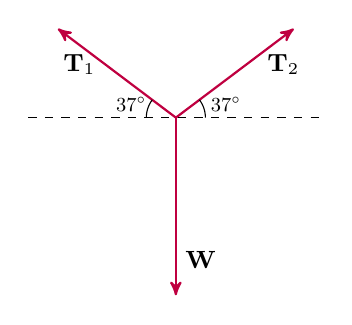
\begin{tikzpicture}[>=latex,xscale=.5*0.15, yscale=.5*0.15][font=\sf\small] 

\draw [purple, thick, ->, >=stealth'](0, 0) -- ({25*cos(37)}, {25*sin(37)})node[black, right, midway, pos=0.6, xshift=4, yshift=0, scale=1]{${\bf T}_2$};

\draw [purple, thick, ->, >=stealth'](0, 0) -- ({25*cos(180-37)}, {25*sin(180-37)})node[black, left, midway, pos=0.6, xshift=0, yshift=0, scale=1]{${\bf T}_1$};

\draw[dashed] (-25, 0) -- (25, 0);

\draw[purple, thick, ->, >=stealth'] (0, 0) -- (0, {-(25*sin(37)+25*sin(180-37))})node[black, right, midway, pos=0.8, xshift=0, yshift=0, scale=1]{${\bf W}$};

\draw[black, samples=100, smooth, domain=0:37, variable=\t] 
		plot ({5*cos(\t)}, {5*sin(\t)}); 

\draw[black, samples=100, smooth, domain=143:180, variable=\t] 
		plot ({5*cos(\t)}, {5*sin(\t)}); 

\node[right, xshift=2, yshift=2, scale=0.8] at ({4*cos(19)}, {4*sin(19)}) {$37^\circ$};

\node[left, yshift=2, scale=0.8] at ({4*cos(161.5)}, {4*sin(161.5)}) {$37^\circ$};


\end{tikzpicture}
\end{document}